%%%%%%%%%%%%%%%%%%%%%%%%%%%%%%%%%%%%%%%%%
% Beamer Presentation
% LaTeX Template
% Version 1.0 (10/11/12)
%
% This template has been downloaded from:
% http://www.LaTeXTemplates.com
%
% License:
% CC BY-NC-SA 3.0 (http://creativecommons.org/licenses/by-nc-sa/3.0/)
%
%%%%%%%%%%%%%%%%%%%%%%%%%%%%%%%%%%%%%%%%%

%----------------------------------------------------------------------------------------
%	PACKAGES AND THEMES
%----------------------------------------------------------------------------------------

\documentclass{beamer}

\mode<presentation> {

% The Beamer class comes with a number of default slide themes
% which change the colors and layouts of slides. Below this is a list
% of all the themes, uncomment each in turn to see what they look like.

%\usetheme{default}
%\usetheme{AnnArbor}
%\usetheme{Antibes}
%\usetheme{Bergen}
%\usetheme{Berkeley}
%\usetheme{Berlin}
%\usetheme{Boadilla}
%\usetheme{CambridgeUS}
%\usetheme{Copenhagen}
%\usetheme{Darmstadt}
\usetheme{Dresden}
%\usetheme{Frankfurt}
%\usetheme{Goettingen}
%\usetheme{Hannover}
%\usetheme{Ilmenau}
%\usetheme{JuanLesPins}
%\usetheme{Luebeck}
%\usetheme{Madrid}
%\usetheme{Malmoe}
%\usetheme{Marburg}
%\usetheme{Montpellier}
%\usetheme{PaloAlto}
%\usetheme{Pittsburgh}
%\usetheme{Rochester}
%\usetheme{Singapore}
%\usetheme{Szeged}
%\usetheme{Warsaw}

% As well as themes, the Beamer class has a number of color themes
% for any slide theme. Uncomment each of these in turn to see how it
% changes the colors of your current slide theme.

%\usecolortheme{albatross}
%\usecolortheme{beaver}
%\usecolortheme{beetle}
%\usecolortheme{crane}
%\usecolortheme{dolphin}
%\usecolortheme{dove}
%\usecolortheme{fly}
%\usecolortheme{lily}
%\usecolortheme{orchid}
%\usecolortheme{rose}
%\usecolortheme{seagull}
%\usecolortheme{seahorse}
%\usecolortheme{whale}
%\usecolortheme{wolverine}

%\setbeamertemplate{footline} % To remove the footer line in all slides uncomment this line
%\setbeamertemplate{footline}[page number] % To replace the footer line in all slides with a simple slide count uncomment this line

%\setbeamertemplate{navigation symbols}{} % To remove the navigation symbols from the bottom of all slides uncomment this line
}

\usepackage{listings}
\usepackage{color}
 
\definecolor{codegreen}{rgb}{0,0.6,0}
\definecolor{codegray}{rgb}{0.5,0.5,0.5}
\definecolor{codepurple}{rgb}{0.58,0,0.82}
\definecolor{backcolour}{rgb}{0.95,0.95,0.92}
 
\lstdefinestyle{mystyle}{
    backgroundcolor=\color{backcolour},   
    commentstyle=\color{codegreen},
    keywordstyle=\color{magenta},
    numberstyle=\tiny\color{codegray},
    stringstyle=\color{codepurple},
    basicstyle=\footnotesize, %\tiny, \small, \footnotesize
    breakatwhitespace=false,         
    breaklines=true,                 
    captionpos=b,                    
    keepspaces=true,                 
    numbers=left,                    
    numbersep=5pt,                  
    showspaces=false,                
    showstringspaces=false,
    showtabs=false,                  
    tabsize=2
}
 
\lstset{style=mystyle}

\usepackage{hyperref}
\usepackage{lipsum}
\usepackage{graphicx} % Allows including images
\usepackage{booktabs} % Allows the use of \toprule, \midrule and \bottomrule in tables

%My personal package
%\usepackage{tikz}

%% Knuths smile box from 
%\centerline{\bf Stable Husbands}
%\bigskip
%\centerline{\sl Donald E. Knuth, Rajeev Motwani, and Boris Pittel}
%\centerline{\sl  Computer Science Department, Stanford University}
\def\pfbox % new experimental version (DEK, November 88)
{{\ooalign{\hfil\lower.06ex % a smiley face
 \hbox{$\scriptscriptstyle -$}\hfil\crcr
 \hfil\lower.7ex\hbox{\"{}}\hfil\crcr
 \mathhexbox20D}}}

%----------------------------------------------------------------------------------------
%	TITLE PAGE
%----------------------------------------------------------------------------------------

\title[PBNP]{Python for Beginners/Non-Programmers} % The short title appears at the bottom of every slide, the full title is only on the title page

\author{Muhammad Izham} % Your name
\institute[Universiti Malaysia Perlis] % Your institution as it will appear on the bottom of every slide, may be shorthand to save space
{
Universiti Malaysia Perlis \\ % Your institution for the title page
\medskip
\textit{izham@unimap.edu.my} \\
\textit{sugita5019@gmail.com} \\ %email

%Check out my templates for simple stuffs

\textit{https://github.com/izham-sugita}
}
\date{} % Date, can be changed to a custom date

\begin{document}

\begin{frame}
\titlepage % Print the title page as the first slide
\end{frame}

\begin{frame}
\frametitle{Overview} % Table of contents slide, comment this block out to remove it
\tableofcontents % Throughout your presentation, if you choose to use \section{} and \subsection{} commands, these will automatically be printed on this slide as an overview of your presentation
\end{frame}

%----------------------------------------------------------------------------------------
%	PRESENTATION SLIDES
%----------------------------------------------------------------------------------------

%------------------------------------------------
\section{The Basics} 

\begin{frame}[fragile]
\frametitle{Before we get started, does anyone want to get out?}
\begin{itemize}
\item Simple paradigm of programming
\begin{itemize}
\item what engineers and scientists care about
\item a lawyer and a cop
\item I will get some of the explanations imprecise
\end{itemize}

\item Programming basic concepts
\begin{itemize}
\item What is it REALLY all about?
	\begin{itemize}
	\item data processing/manipulations
	\item programming is a process/steps of processing/manipulating data
	\end{itemize}

\item What is the most basic types of data?
	\begin{itemize}
	\item characters/strings
	\item number/numerics $\longrightarrow$ float/integer
	\end{itemize}

\end{itemize}

\end{itemize}

\end{frame}
\begin{frame}[fragile]
\frametitle{Before we get started, does anyone want to get out?}
\begin{figure}
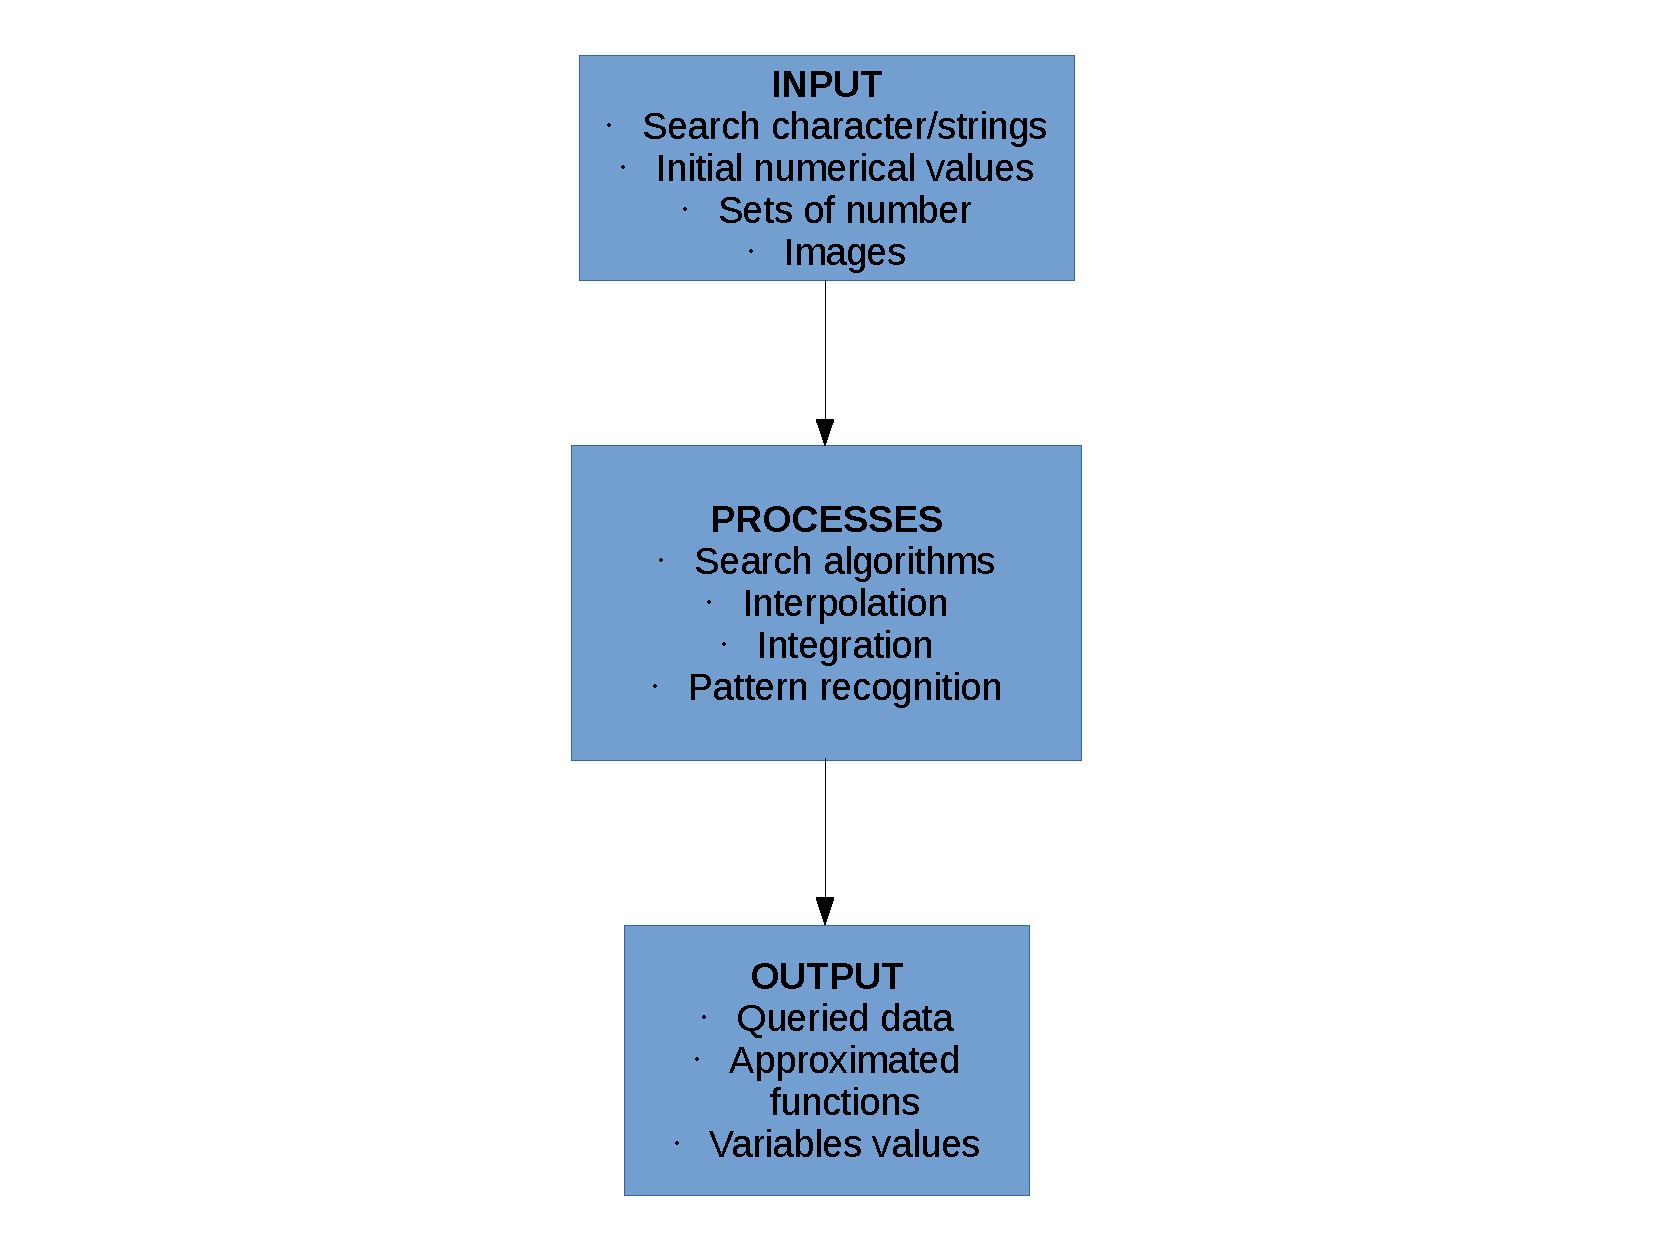
\includegraphics[width=0.8\linewidth]{ProgrammingFlow.pdf}
\end{figure}
\end{frame}
\begin{frame}[fragile]
\frametitle{Before we get started, does anyone want to get out?}

\begin{itemize}
\item Coding paradigm
	\begin{itemize}
	\item programming language == English (sorry, Mandarin not required)
	\item syntax is based on English
	\item coding is a reduction of English instructions
	\end{itemize}

\item Syntax must be remembered
	\begin{itemize}
	\item read the manual $\longrightarrow$ documentations are vital
	\item memorize THE MOST COMMONLY USED syntax only
	\item good algorithm will always beats bad algorithm
	\end{itemize}		

\item I don't remember every syntax so you have to bare with me $\LARGE \pfbox$

\end{itemize}

\end{frame}


\begin{frame}
\frametitle{Installation}

\begin{itemize}
\item Download from \url{https://www.python.org/}
\item For Ubuntu download from repository:\lstinputlisting[language=bash, firstline=1, lastline=1, numbers=none]{./install-commands.txt}

\item For Windows, download from \url{https://www.python.org/downloads/windows/}

\item For Ubuntu installing packages:\lstinputlisting[language=bash, firstline=2, lastline=2, numbers=none]{./install-commands.txt}

\item For Windows installing packages if $C:\backslash Python\backslash Scripts \backslash$ is in the path:\lstinputlisting[language=bash, firstline=3, lastline=3, numbers=none]{./install-commands.txt}

\item For Windows installing packages:\lstinputlisting[language=bash, firstline=4, lastline=4, numbers=none]{./install-commands.txt}

%C:\Python\Scripts

\end{itemize}

\end{frame}


\begin{frame}
\frametitle{Installation}

\begin{itemize}
\item For Windows, the default editor is IDLE
\begin{figure}
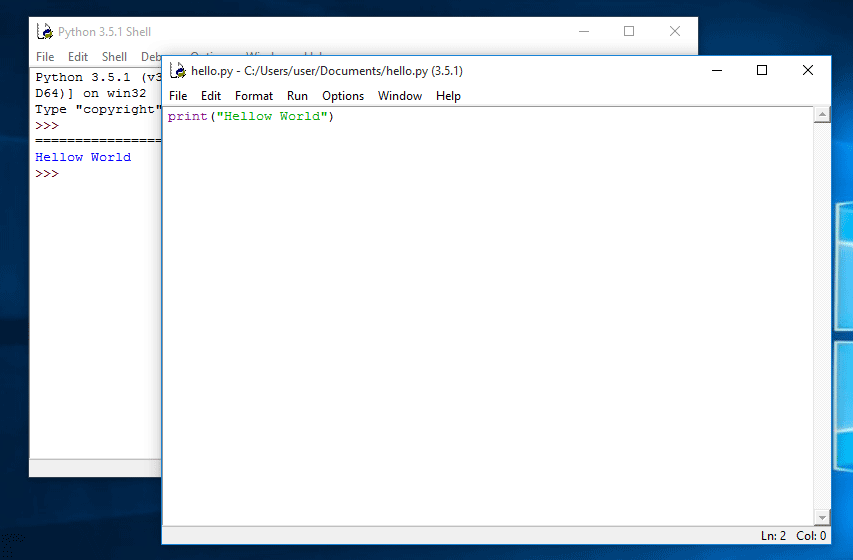
\includegraphics[width=0.8\linewidth]{IDLE.png}
\end{figure}
\end{itemize}

\end{frame}


% Sections can be created in order to organize your presentation into discrete blocks, all sections and subsections are automatically printed in the table of contents as an overview of the talk
%------------------------------------------------

%\subsection{Subsection Example} % A subsection can be created just before a set of slides with a common theme to further break down your presentation into chunks

\begin{frame}
\frametitle{Introduction}
%\lipsum[1]

\begin{itemize}
\item Created by: Guido van Rossum, 1989-1991
\item Why: The creator wanted something easy to use.
\item Is it really that easy? Yes (and no)
\item Very readable with little memory managment.
\item Lots of proven libraries. Open source.
\item \url{https://docs.python.org/3/tutorial/index.html}
\item \url{https://www.tutorialsteacher.com/python}
\item \url{https://www.w3schools.com/python/default.asp}
\end{itemize}

\end{frame}


\begin{frame}[fragile]
\frametitle{The Zen of Python}
\begin{itemize}
\tiny
\item Beautiful is better than ugly.
\item Explicit is better than implicit.
\item Simple is better than complex.
\item Complex is better than complicated.
\item Flat is better than nested.
\item Sparse is better than dense.
\item Readability counts.
\item Special cases aren't special enough to break the rules.
\item Although practicality beats purity.
\item Errors should never pass silently.
\item Unless explicitly silenced.
\item In the face of ambiguity, refuse the temptation to guess.
\item There should be one -- and preferably only one -- obvious way to do it.
\item Although that way may not be obvious at first unless you're Dutch.
\item Now is better than never.
\item Although never is often better than *right* now.
\item If the implementation is hard to explain, it's a bad idea.
\item If the implementation is easy to explain, it may be a good idea.
\item Namespaces are one honking great idea -- let's do more of those! 
\end{itemize}

\end{frame}


%------------------------------------------------
\section{Python3 Coding}
%------------------------------------------------

\begin{frame}[fragile]
\frametitle{The "Hello, World!"}
Greetings!!
\lstinputlisting[language=Python, firstline=4]{../helloPython.py}

file: helloPython.py
\end{frame}
\begin{frame}[fragile]
\frametitle{Variables size}
In Python:
\newcommand{\newfilename}{py-number.py}

\lstinputlisting[language=Python, firstline=1, lastline=12]{../py-number.py}

file: \newfilename
\end{frame}

\begin{frame}[fragile]
\frametitle{Variables size}
In C/C++/Fortran:
\newcommand{\newfilename}{datasize.c}

\lstinputlisting[language=C, firstline=1, lastline=14]{../datasize.c}

file: \newfilename
\end{frame}

\begin{frame}[fragile]
\frametitle{Variables size}
\begin{itemize}
\item In Python, int=28, long int=32, float=32, double=32 bytes.
\item Generally a lot more than standard programming language; why?
\item In C/C++/Fortran int=4, long int=8, float=4, double=8 bytes
\item Curious?
\end{itemize}

\end{frame}
\begin{frame}[fragile]
\frametitle{Variables in Python3}
Importing a module:
\lstinputlisting[language=Python, firstline=1, lastline=1]{../variables.py}

Print to screen:
\lstinputlisting[language=Python, firstline=2, lastline=5]{../variables.py}

Taking an input:
\lstinputlisting[language=Python, firstline=7, lastline=8]{../variables.py}

file: variables.py
\end{frame}

\begin{frame}[fragile]
\frametitle{Variables in Python3}
How to use module:
\lstinputlisting[language=Python, firstline=10]{../variables.py}

file: variables.py
\end{frame}
\begin{frame}[fragile]
\frametitle{Repetitive task}

\begin{itemize}
\item Loop 
\lstinputlisting[language=Python, firstline=11, lastline=16]{../py-loop.py}
\end{itemize}

\end{frame}

\begin{frame}[fragile]
\frametitle{Repetitive task}

\begin{itemize}
\item Loop with string data.
\lstinputlisting[language=Python, firstline=24, lastline=26]{../py-loop.py}
\end{itemize}

\end{frame}
\begin{frame}[fragile]
\frametitle{Control: Asking to do things}
\newcommand{\newfilename}{py-control.py}

\begin{itemize}
\item Simple control.
\lstinputlisting[language=Python, firstline=1, lastline=3]{../py-control.py}
\end{itemize}

file: \newfilename

\end{frame}

\begin{frame}[fragile]
\frametitle{Control: Asking to do things}
\newcommand{\newfilename}{py-control.py}

\begin{itemize}
\item Nested if-elif
\lstinputlisting[language=Python, firstline=7, lastline=15]{../py-control.py}
\end{itemize}


file: \newfilename

\end{frame}
\begin{frame}[fragile]
\frametitle{Container: List, Dictionaries, Set, Tupples}
\newcommand{\newfilename}{python-container.py}
Container: List
\begin{itemize}
\item A list can contains any type of variable
\item Unlike the normal practice of array where an array contains just one type of variable
\end{itemize}
\lstinputlisting[language=Python, firstline=2, lastline=6]{../python-container.py}

file: \newfilename
\end{frame}
\begin{frame}[fragile]
\frametitle{Class in Python3}
\begin{itemize}
\item Variables in class are public by default.
\end{itemize}
Defining a class:
\lstinputlisting[language=Python, firstline=1, lastline=10]{../py-class0.py}
file: py-class0.py
\end{frame}

%---------------------------------------------------------------------------

\begin{frame}[fragile]
\frametitle{Class in Python3}
\begin{itemize}
\item Variables can be made private.
\end{itemize}
Defining a class:
\lstinputlisting[language=Python, firstline=33, lastline=37]{../py-class0.py}
file: py-class0.py
\end{frame}

%---------------------------------------------------------------------------

\begin{frame}[fragile]
\frametitle{Class in Python3}
\begin{itemize}
\item Initiating class.
\end{itemize}
\lstinputlisting[language=Python, firstline=1, lastline=10]{../py-class1.py}
file: py-class1.py
\end{frame}

%---------------------------------------------------------------------------
\begin{frame}[fragile]
\frametitle{Function: Modularizing your codes}
\newcommand{\newfilename}{py-function.py}

\lstinputlisting[language=Python, firstline=2, lastline=6]{../py-function.py}

file: \newfilename
\end{frame}

%------------------------------------------------------------------------------

\begin{frame}[fragile]
\frametitle{Function: Modularizing your codes}
\newcommand{\newfilename}{py-function.py}
\begin{itemize}
\item Creating a function that change the value of its input: 

\lstinputlisting[language=Python, firstline=44, lastline=46]{../py-function.py}

\item Function parameters in Python are pass-by-reference.
\item To change the value $\longrightarrow$ mutable object as input parameter e.g. list, numpy's array

\end{itemize}

file: \newfilename
\end{frame}

%-----------------------------------------------------------------------------

\begin{frame}[fragile]
\frametitle{Function: Modularizing your codes}
\newcommand{\newfilename}{py-function.py}
\begin{itemize}
\item Creating a function that change the value of its input: 

\lstinputlisting[language=Python, firstline=53, lastline=55]{../py-function.py}

\item Input parameters as numpy's array.

\lstinputlisting[language=Python, firstline=74, lastline=82]{../py-function.py}

\end{itemize}

file: \newfilename
\end{frame}

%-----------------------------------------------------------------------------

\section{Practical Implementations}

\begin{frame}[fragile]
\frametitle{Matplotlib module}

\begin{itemize}
\item Very efficient module for plotting almost everything.
\item Capable for plotting graphs and images.
\item Documentation from \url{https://matplotlib.org/3.1.0/index.html}
\end{itemize}

\newcommand{\newfilename}{py-matplotlib.py}
\lstinputlisting[language=Python, firstline=1, lastline=7]{../py-matplotlib.py}
file: \newfilename

\end{frame}

%-------------------------------------------------------------------------------

\begin{frame}[fragile]
\frametitle{NumPy module}

\begin{itemize}
\item Specific module for numerical simulations.
\item Very excellent for array manipulation.
\item Documentation from \url{https://www.numpy.org/}
\end{itemize}

%\newcommand{\newfilename}{py-matplotlib.py}
%\lstinputlisting[language=Python, firstline=1, lastline=7]{../py-matplotlib.py}
%file: \newfilename

\end{frame}

%-------------------------------------------------------------------------------

\begin{frame}[fragile]
\frametitle{SciPy module}

\begin{itemize}
\item Scientific calculations module.
\item Lots of functions for scientific computation.
\item Documentation from \url{https://www.scipy.org/}
\item Specific manuals \url{https://docs.scipy.org/doc/scipy-1.3.0/reference/}
\end{itemize}

%\newcommand{\newfilename}{py-matplotlib.py}
%\lstinputlisting[language=Python, firstline=1, lastline=7]{../py-matplotlib.py}
%file: \newfilename

\end{frame}

%--------------------------------------------------------------------------------

\begin{frame}[fragile]
\frametitle{Standard template}
\begin{itemize}
\item This is a standard template slide.
\item Modify by adding items.
\end{itemize}

\end{frame}
\begin{frame}
\Huge{\centerline{Thank You!}}
\Huge{\centerline{Questions?}}
\end{frame}

\end{document} 